\begin{frame}{$\cos\theta_{CM}$ of $p_{K^-}-p_{n_{missing}}$ vs $"n" momentum$}
  \centering
  $d(K^-, n \pi^+ \pi^-)"n"$ was only selected. (No invariant mass $\Sigma$ selection).\\
  \vspace{3mm}
  \footnotesize
  1-step reaction : $K^-d\rightarrow \pi^{\mp} \Sigma^{\mp} "n_{spectator}"$\\
  \scriptsize
  $K^-p\rightarrow \pi^{\mp}\Sigma^{\pm}$ angular dist. were simulated using previous experimental data.
  
  
  \tminipageThree{
    \begin{figure}
      \scriptsize
      Data\\
      \includegraphics[width=3cm]{../pic/Run78/noumi/cos_piS_f_CM_mmN_mom_data.eps}
    \end{figure}
  }{
    \begin{figure}
      \scriptsize
      1-step $\pi^-\Sigma^+$(Forward)\\
      \includegraphics[width=3cm]{../pic/Run78/noumi/cos_piS_f_CM_mmN_mom_1step_Sp.eps}
    \end{figure}
  }{
    \begin{figure}
      \scriptsize
      1-step $\pi^+\Sigma^-$(Forward)\\
      \includegraphics[width=3cm]{../pic/Run78/noumi/cos_piS_f_CM_mmN_mom_1step_Sm.eps}
    \end{figure}
  }
  
  \tminipageThree{
    \centering
    \footnotesize
    2-step $\pi^{\mp}\Sigma^{\pm}$ reaction\\
    \scriptsize
    \vspace{1mm}
    $K^-$ kick out neutron and recoiled $\bar{K}$ reacts with $N$.
    \vspace{1mm}
    $K^-d \rightarrow n \pi^{\pm}\Sigma^{\mp}$ $\theta_n<8$ degree\\
    \tiny
    $m_{\pi\Sigma}$ : Flat $\pi\Sigma$ thre. $\sim$ 1.8 $[GeV/c^2]$  

  }{
    \begin{figure}
      \scriptsize
      2-step $\pi^-\Sigma^+$(Backward)\\
      \includegraphics[width=3cm]{../pic/Run78/noumi/cos_piS_f_CM_mmN_mom_2step_Sp.eps}
    \end{figure}
  }{
    \begin{figure}
      \scriptsize
      2-step $\pi^+\Sigma^-$(Backward)\\
      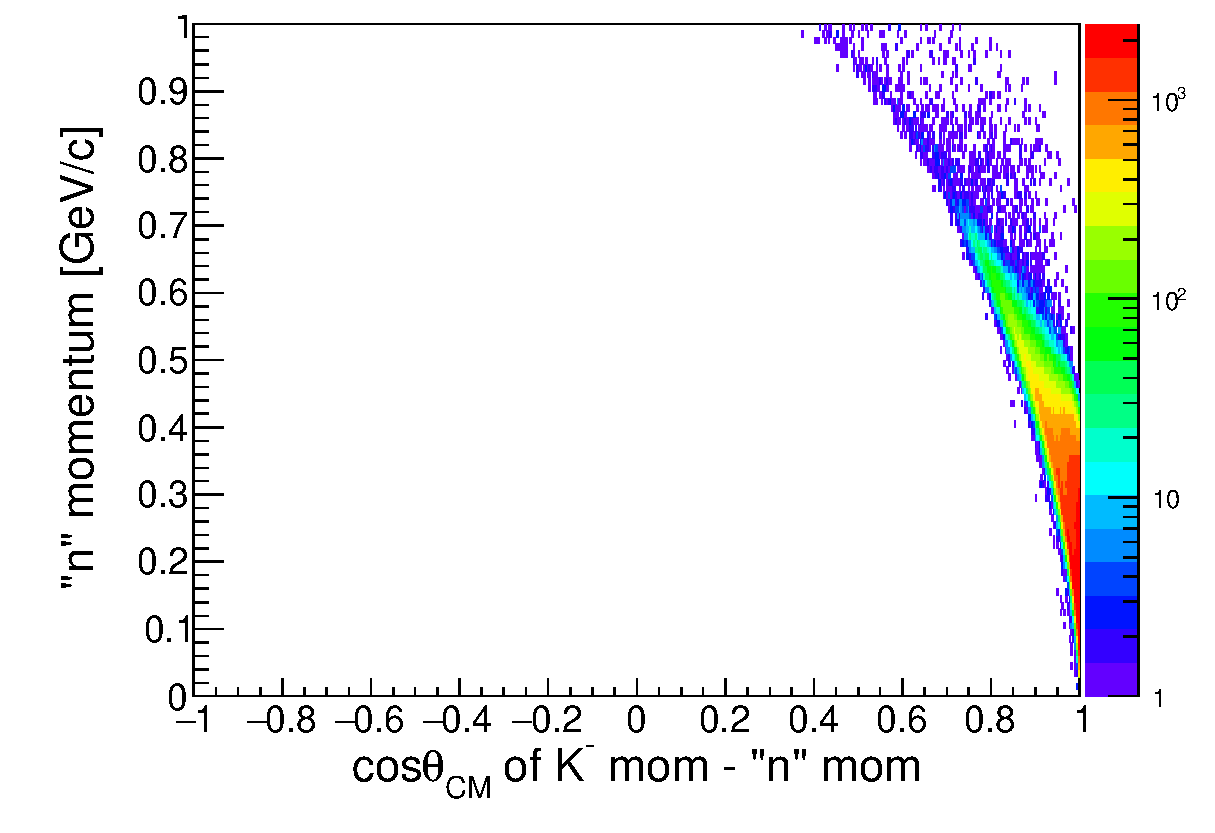
\includegraphics[width=3cm]{../pic/Run78/noumi/cos_piS_f_CM_mmN_mom_2step_Sm.eps}
    \end{figure}
  }
  \centering
  \large
  No events, $n_{detected}$ come from $\Sigma$ decay in 2-step events.

\end{frame}
